\title{Graphenisomorphie in quasipolynomieller Zeit\\ Der Algorithmus von L\'{a}szl\'{o} Babai}
\author{Yussuf Kassem
        \and
        Benjamin Deutz
        }
\documentclass[a4paper]{article}
\usepackage[ngerman]{babel}
\usepackage[utf8]{inputenc}
\usepackage[T1]{fontenc}
\usepackage{amsmath}
\usepackage{graphicx}
\usepackage{tikz}
\usetikzlibrary{arrows} 
\tikzset{knoten/.style={circle,fill=black,inner sep=1mm}}
\usepackage[section]{placeins}
\usepackage{url}
\usepackage{hyperref}

\usepackage{graphicx}

\newtheorem{theorem}{Theorem}
\newtheorem{example}{Beispiel}
\newtheorem{lemma}{Lemma}
\newtheorem{proposition}{Proposition}
\newtheorem{scolium}{Scolium}   %% And a not so common one.
\newtheorem{definition}{Definition}
\newenvironment{proof}{{\sc Proof:}}{~\hfill QED}
\newenvironment{AMS}{}{}
\newenvironment{keywords}{}{}

%Quellen
\newcommand{\babai}{\url{http://people.cs.uchicago.edu/~laci/CV13.pdf}}
\newcommand{\babaipublications}{\url{http://people.cs.uchicago.edu/~laci/pub/pub.pdf}}
\newcommand{\wlcoloring}{\url{https://simons.berkeley.edu/sites/default/files/docs/5854/mainhandout.pdf}}



\begin{document}
\newpage
\maketitle
\begin{abstract}
Dieses Dokument ist im Rahmen des Kurses \glqq Panorama der Mathematik - Seminar über Fehler\grqq\ im an der Freien Universität Berlin im Sommersemester 2017 entstanden. Es beinhaltet die Ausarbeitung eines Vortrags vom 10. Juli 2017 zum Thema \glqq Graphenisomorphie in quasipolynomieller Zeit\grqq. Dabei wird insbesondere die zeitliche Abfolge der Ereignisse nach der Ankündigung Babais einen quasipolynomiellen Algorithmus gefunden zu haben dargestellt. Das Ziel besteht darin, die Vortragsstruktur und die Inhalte des Themas abzubilden. \end{abstract}

\section{Definitionen}
In diesem Kapitel werden wir die Einstiegsdefinitionen und Notationen festhalten, die für den Vortrag zentral sind.
\begin{definition}
	Ein Graph $G$ ist ein geordnetes Paar $(V, E)$. Dabei ist $V$ eine Menge, deren einzelnen Elemente wir Knoten nennen. $E$ ist die Menge aller Kanten. Jede Kante besteht aus $2$ verschiedenen Knoten.
\end{definition}

\begin{definition}
Gegeben seien zwei Graphen $G = (V,E)$ und $G' = (V',E')$. Dann gilt $G\cong G' \Leftrightarrow \exists \varphi:V\rightarrow V'$ ist eine bijektive Abbildung, für die gilt: $\{v,w\}\in E \Leftrightarrow \{\varphi(v),\varphi(w)\}\in E'$. Wir sagen dann, dass $G$ und $G'$ isomorph zueinander sind. Wir nennen $\varphi$ einen Isomorphismus.
\end{definition}

Diese Definitionen werden im Folgenden an zwei Beispielen anschaulich gemacht. Dazu schauen wir uns zuerst die beiden Graphen in Abbildung \ref{fig:isomorph} an. Durch die Angabe einer Abbildung $\varphi$ kann man erkennen, dass es sich um zwei isomorphe Graphen handelt. Die Abbildung $\varphi$ ist im Folgenden angegeben.

$$\varphi =
    \begin{cases}
    \varphi(a) = 1, \varphi(b) = 6,
    \varphi(c) = 8, \varphi(d) = 3\\
    \varphi(g) = 5, \varphi(h) = 2,
    \varphi(i) = 4, \varphi(j) = 7\\
    \end{cases}  
$$

\begin{figure}
\centering
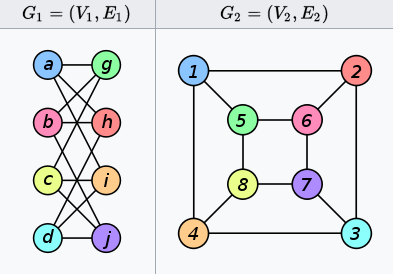
\includegraphics[scale=0.8]{isomorph.png}
\caption{Zwei isomorphe Graphen}\label{fig:isomorph}
\end{figure}


Ein weiteres Beispiel zeigt, dass zwei Graphen, obwohl sie sich auf den ersten Blick vielleicht recht ähnlich sehen, nicht unbedingt isomorph sein müssen. In Abbildung \ref{fig:nisomorph} sehen wir ebenfalls zwei Graphen. Beide haben $5$ Knoten und $6$ Kanten. Um nun argumentieren zu können, warum diese beiden Graphen nicht isomorph sind, brauchen wir eine neue Definition.

\begin{definition}
Gegeben sei ein Graph $G = (V,E)$. Sei $v\in V$ ein beliebiger Knoten. Wir definieren $$d_G(v) := \sum_{e\in E, v\in e} 1.$$
Wir nennen $d_G(v)$ den Grad von $v$. Anders ausgedrückt ist der Grad also die Anzahl aller Kanten, die $v$ mit anderen Knoten verbinden.
\end{definition}

Es ist offensichtlich, dass bei einer isomorphen Abbildung Knoten mit Grad $x$ auf Knoten mit Grad $x$ abgebildet werden müssen.
Wenn wir die Grade aller Knoten in den beiden Graphen betrachten, bemerken wir, dass beide Graphen $3$ Knoten mit Grad $2$ und $2$ Knoten mit Grad $3$ besitzen. Im linken Graphen sind die beiden Knoten mit Grad $3$, nämlich c und d, miteinander verbunden. Im rechten Graphen allerdings sind die beiden Knoten mit Grad $3$ nicht verbunden. Dieses Argument reicht aus, um zu zeigen, dass die beiden Graphen nicht isomorph sein können. 

\begin{figure}
\centering
\begin{tikzpicture}[>=stealth]
    \path node [knoten, label=below:a] (1) at (0,0) {}
          	node [knoten, label=below:b] (2) at (3,0)  {}
          	node [knoten, label=right:c] (3) at (3,3)  {}
          	node [knoten, label=left:d] (4) at (0,3)  {}
          	node [knoten, label=above:e] (5) at (1.5,5)  {}
          	
	     (1) edge (2)
	     (2) edge (3)
	     (1) edge (4) 
	     (3) edge (4)
	     (3) edge (5)
	     (4) edge (5);
	     
	     \path node [knoten, label=below:1] (6) at (7,0) {}
	      node [knoten, label=below:2] (7) at (10,0) {}
	      node [knoten, label=right:3] (8) at (10,3) {}
	      node [knoten, label=left:4] (9) at (7,3) {}
	      node [knoten, label=above:5] (10) at (8.5,5) {}
          		
	     (6) edge (8)
	     (6) edge (9)
	     (9) edge (10)
	     (8) edge (10)
	     (9) edge (7)
	     (7) edge (8)
	     
	     ;
  \end{tikzpicture}
  \caption{Zwei nicht isomorphe Graphen}\label{fig:nisomorph}
  \end{figure}



\section{L\'{a}szl\'{o} Babai}
L\'{a}szl\'{o} Babai ist ein in Ungarn geborener Mathematiker. Er ist 1950 in Budapest geboren und U.S.-Staatsbürger. Er ist Professor für Mathematik und Informatik an der Universität von Chicago und beschäftigt sich vornehmlichn mit Kombinatorik, Algorithmentheorie und Komplexitätstheorie. Seine Reputation weißt inzwischen über 200 akademische \emph{papers} auf (Stand: Juli 2017).\footnote{Vgl.\hspace{0.1cm}\babai} \footnote{Vgl. \babaipublications}

\section{Geschichte der Graphenisomorphie} \label{sec:historical}

In diesem Teil möchten wir einen kleinen historischen Überblick über Ergebnisse im Bereich der Graphenisomorphie geben. Dies schließt die neuesten Erkenntnisse Babais mit ein.
\subsection{Historisches}

\subsection{Babais Durchbruch}

Im September 2015
\section{Standardheuristiken im Algorithmus und Probleme}
In den folgenden drei Unterkapiteln wollen wir zwei Standardheuristiken und eine Gruppe von Graphen vorstellen, bei denen diese Standardheuristiken problematisch sind. Weiterhin bildet das zweite Unterkapitel die Grundlage für einen Teil der später in dieser Arbeit besprochenen Komplexitätsanalyse.

\subsection{Färbung}
Färbung bedeutet im Bereich der Graphentheorie im Allgemeinen eine besondere Art des Markierens. Dabei unterscheidet man zwischen gültigen und nicht gültigen Färbungen. Die Gültigkeit entscheidet sich dadurch, ob zwei benachbarte Knoten eine gemeinsame Farbe besitzen. Tun sie dies, ist die Färbung nicht gültig. Wir beschäftigen uns in dieser Ausarbeitung jedoch nicht mit gegebenen Färbungen von Graphen, sondern mit einem Algorithmus, der eine Färbung erzeugt. Wie im Kapitel \glqq\nameref{sec:historical}\grqq\ bereits erwähnt gibt es k-dimensionale Weisfeiler-Leman Algorithmen. Wir fokussieren uns hier auf den 1-dimensionalen Fall, den man auch \emph{colour refinement} nennt.

Der Algorithmus startet dabei auf einem Graphen, bei dem alle Knoten dieselbe Farbe haben. Anschließend beginnt einer Abfolge von Schritten, bei denen man zwei beliebige Knoten $v, w$ und die Anzahl der jeweiligen Nachbarn mit der gleichen Farbe betrachtet. Wenn eine Farbe $c$ existiert, sodass $v$ und $w$ eine verschiedene Anzahl von Nachbarn mit der Farbe $c$ haben, dann erhalten $v$ und $w$ verschiedene Farben. Wichtig ist in diesem Zusammenhang, dass die neuen Färbungen erst am Ende der gesamten Abfolge gemacht werden. Um sich dies verdeutlichen zu können sei an dieser Stelle festgehalten, dass nach der ersten Abfolge von Schritten eine Färbung entsteht, die den Grad jedes Knoten bestimmt. Diese Abfolge wird nun sooft wiederholt, bis die Färbung stabil ist, d.h. keine Farbänderungen mehr auftreten. 

Diese Färbungen sind ein erster Schritt, um zwei gegebene Graphen auf Isomorphie zu untersuchen. Gegeben seien zwei Graphen $G$ und $G\rq{}$ auf denen stabile Färbungen durch unseren Algorithmus entstanden sind. Diese Färbungen können nun auf Isormophie untersucht werden. Sind die Färbungen nicht isomorph, dann sind es auch die Graphen nicht. Die Umkehrung gilt jedoch im Allgemeinen nicht. Weiterhin kann Färbung natürlich auch genutzt werden, um die Anzahl der zu untersuchenden Abbildungen zu reduzieren, da nur entsprechend gefärbte Knoten in $G$ auf entsprechend gefärbte Knoten in $G\rq{}$ abgebildet werden können.\footnote{Vgl. \wlcoloring} 

\subsection{Individualisierung}
Färbungen nutzen die Strukturen, die bereits auf einem Graphen gegeben sind. Es gibt jedoch Graphen auf denen Färbungen zwar stabil sind, aber uns keinen Schritt weiterbringen. Dabei handelt es sich um reguläre Graphen.
\begin{definition}
Gegeben sei ein Graph $G = (V,E)$. Wenn alle Knoten aus $V$ denselben Grad haben, nennen wir den Graphen $G$ regulär.
\end{definition}
Dies möchten wir nun an einem bekannten Beispiel visualisieren. Außerdem wird im Kapitel \nameref{sec:complexity} auf dieses Beispiel zurückgegriffen. 

Wir betrachten den sogenannten Petersen-Graphen, den wir auch in Abbildung \ref{fig:petersen} sehen. Da dieser regulär ist, hilft uns eine Färbung nicht weiter. Um dieses Problem anzugreifen \emph{individualisieren} oder färben wir nun einen Knoten und benutzen anschließend dieselbe Funktiuonalität wie beim Algorithmus der Färbung. Hier brauchen wir jetzt ein Bild...

\begin{figure}
\centering
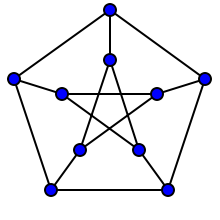
\includegraphics[scale=0.8]{petersen.png}
\caption{Der Petersen-Graph}\label{fig:isomorph}
\end{figure}

\subsection{Johnson-Graphen}
Kurze Erklärung was Johnson Graphen sind und das deren hohe Symmetrie zu Problemen bei der Färbung führt. Alles aus dem VIdeo von Babai zitieren mit Zeitangaben!

\begin{figure}
\centering
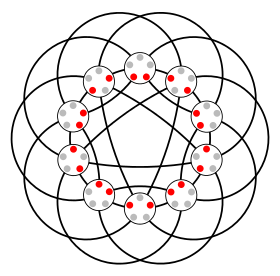
\includegraphics[scale=0.8]{j52.png}
\caption{Der Johnson-Graph $J(5,2)$}\label{fig:j52}
\end{figure}

\section{Einordnung in die Komplexitätsklassen}\label{sec:complexity}


\section{Quellen}

\begin{thebibliography}{9}
     \bibitem{MyFavorite}
         {\sc Lamport, L.,}
         ``\LaTeX - A Document Preparation System'',
         Addison-Wesley, 1998.

    \bibitem{BobsPaper}
         {\sc Fillioque R.} and {\sc Heliotrope, B.,}
         {\em Why Fermat's last theorem is really a lemma,}
         American Mathematical Weekly,
         Vol. 7, No. 1, pp 115-116, 1998.

\end{thebibliography}
\end{document}
